\documentclass[journal, a4paper]{IEEEtran}
\usepackage{graphicx}   
\usepackage{url}        
\usepackage{amsmath}   
\usepackage[english]{babel}
\usepackage{amsmath,amssymb,amsfonts}
\usepackage{float}
\usepackage{listings}
\begin{document}


	\title{Time Series Analysis and Forecasting \\2DD23}
	\author{Xuqiang Fang\quad x.fang@student.tue.nl\\ Hadi Sotudeh\quad h.sotudeh@student.tue.nl}
	\markboth{Eindhoven University of Technology}{}
	\maketitle

\begin{abstract}
% Time series is a series of data points indexed in time order. Time series analysis comprises methods for analyzing time series data in order to extract meaningful statistics and other characteristics of the data, time series  forecasting is the use of a model to predict future values based on previously observed values.\cite{time_series} 
Time series is a series data points with time order indexes. Researches have been focused on analyzing time series and building models in order to extract meaningful characteristics from it. Time series forecasting is to use models to predict future values according to previously observed values. This report consists of time series analysis and forecasting, using different models such as Holt-Winter's model and Box-Jenkins model, based on the same criterion, the best model is selected and used to forecast future values. It shows that even if the model can fit the time series well, there are still some incidents which can affect the precision of the forecast by the model.
\end{abstract}

\section{Introduction}
Part I is an univariate time series analysis, starting with exploratory data analysis (EDA), both in time domain and frequency domain, based on the EDA we identified the possible trend and seasonality, then we performed Holt-Winter's exponential smoothing, automatic exponential smoothing as well as Box-Jenkins model to fit the time series. Using the criteria AICc (SSE for Holt-Winter's) we selected the best model, and then we forecasted the future with the model. 

Part II is the analysis of multivariate time series. We also started with EDA, for the energy per capita time series, we identified that there was trend but no seasonal patterns, and we continued with frequency domain analysis. Then we tried to fit an ARIMA model for the energy per capita. For the dynamic regression, we tried to use one of the time series to forecast another. Finally we fit an exponential smoothing model to the energy per capita time series.

Verification and validation are useful when building models. We performed both verification and validation on all models and we forecast future with the model that performed the best.
% Verification and validation are both very important in building models. Validation assures that the model we fit is going to capture the specifications of the time series while verification assures that the model we fit is able to meet the requirements. \\
% \textit{WHAT?}
% Validation helps find the best type of tools and verification helps find the suitable size of the tool!
\section{Part I}


Starting with the exploratory data analysis both in the time domain and the frequency domain, we first transformed the dataset into time series, then we plotted it in time domain, as shown in figure \ref{fig1:data_ts}, we found out that there were seasonal patterns and missing values (from March 1995 to September 1996), and there were maybe trends within the time series. Each year, the level goes up first and then goes down, and that is the seasonal pattern.


To see if the successive observations are correlated, we plotted the autocorrelation plot at time lag 1, and calculated the coefficient. We obtained $R=0.734108908 $, which shows that at time lag 1, the successive observations are positively correlated as shown in figure \ref{fig1:successive}.

\subsection{Exploratory Data Analysis}
\begin{figure}[H]
\begin{center}
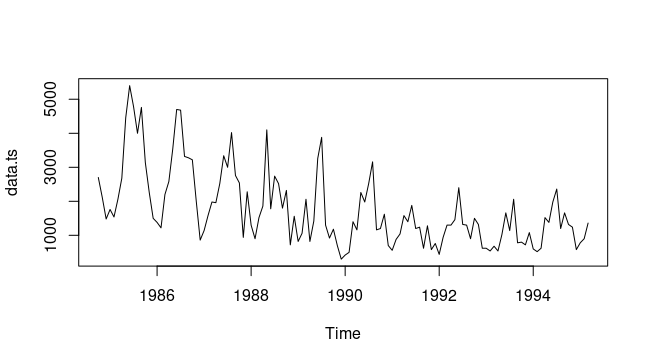
\includegraphics[scale=0.45]{fig1/data_ts.png}
\caption{Time Series Plot}
\label{fig1:data_ts}
\end{center}
\end{figure}

Then we continued with the analysis both in time domain and frequency domain.
\begin{figure}[H]
\begin{center}
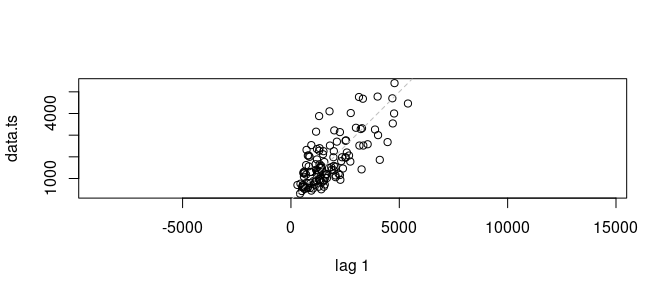
\includegraphics[scale=0.4]{fig1/successiveRelations.png}
\caption{Autocorrelation at time lag 1}
\label{fig1:successive}
\end{center}
\end{figure}



In the time domain, as shown in figure \ref{fig1:tsdisplay}, we can identify seasonality in ACF plot because after each 12 months, the pattern is repeated (but it is not clear whether or not it is an additive seasonality). For the trend, we concluded that there was a weak decreasing trend if any trend existed, because we did not see a lot of high values for the ACF plot. Also from the PACF plot, we can see that successive observations are positively correlated. Also from the log transformed time series plot,  we found out an irregular fluctuations around year 1990.\\
In the frequency domain, we started with the raw periodogram and then followed by the smoothed periodogram. From the raw periodogram we can see that there are multiple peaks within the periodogram but there seems no dominant frequencies within the periodogram.


\begin{figure}[H]
\begin{center}
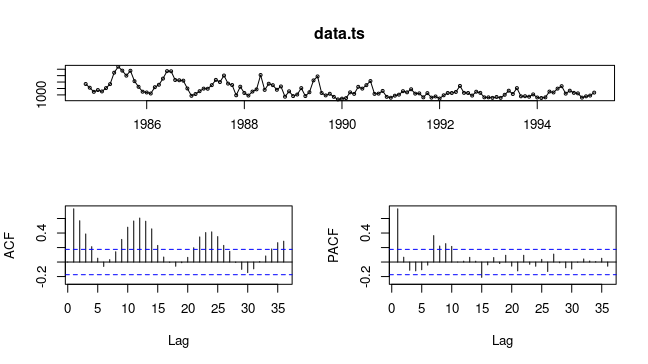
\includegraphics[scale=0.4]{fig1/data_tsdisplay.png}
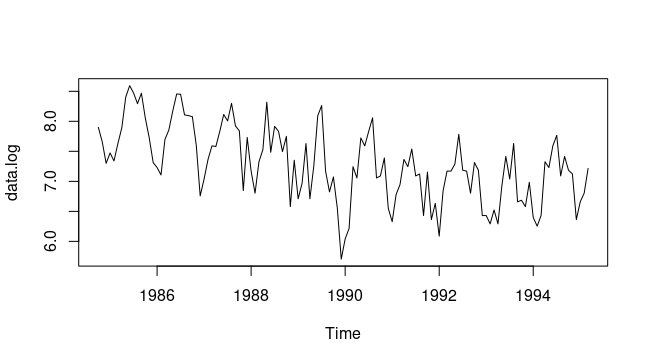
\includegraphics[scale=0.4]{fig1/data_log.png}
\caption{Time Domain: tsdisplay and log transformed data}
\label{fig1:tsdisplay}
\end{center}
\end{figure}



\begin{figure}[H]
\begin{center}
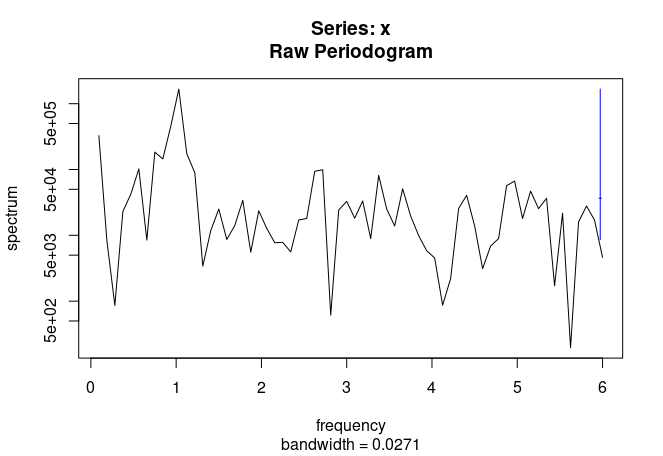
\includegraphics[width=0.3\textwidth]{fig1/frequncyPlot.png}
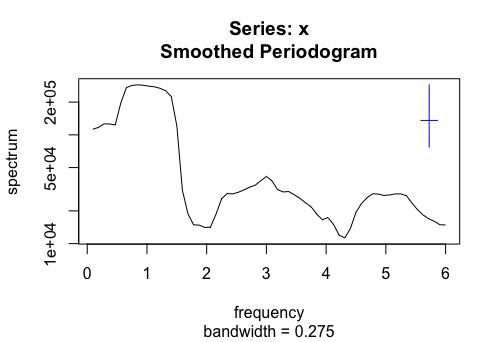
\includegraphics[width=0.3\textwidth]{fig1/smooth.png}
\caption{Frequency Domain: Raw and smoothed periodogram}
\label{fig1:frequency}
\end{center}
\end{figure}

Then we continued with the smoothed periodogram and we found that there is a dominant frequency around 1, which is the monthly record of the data, which suggests that there are seasonal patterns within the time series because of the the low frequency part in the spectrum which is high.

\subsection{Seasonal Decomposition}
Based on Hyndman's book,  'If the data have a strong seasonal pattern, we recommend that seasonal differencing be done first because sometimes the resulting series will be stationary and there will be no need for a further first difference.' \cite{fpp}.\\
By looking at the time series, we found out there was a yearly seasonal pattern, within each year, the level goes up in January and then goes down after June, it reaches a low point in December. The level goes up quite smoothly with barely some small vibrations.
Since a seasonal pattern was detected, we proceeded with seasonal decomposition of the time series. First we performed one time seasonal differencing, and we obtained the results as shown in figure \ref{fig1:seasonal}. From the ACF and PACF plots, we identified that there were still some significant autocorrelations within the plots, so we continued with another seasonal differencing and we found out that the significant patterns still existed and were about the same. So we figured out that one time seasonal decomposition was enough.\\
To decide if the seasonal pattern is additive or multiplicative, we looked at the seasonal variation to see if it was constant over time or not. And we found out that the seasonal variation was proportional to the trend, as shown in figure \ref{fig1:data_ts}, so we concluded that the seasonal pattern was \textbf{multiplicative}.

\begin{figure}[H]
\begin{center}
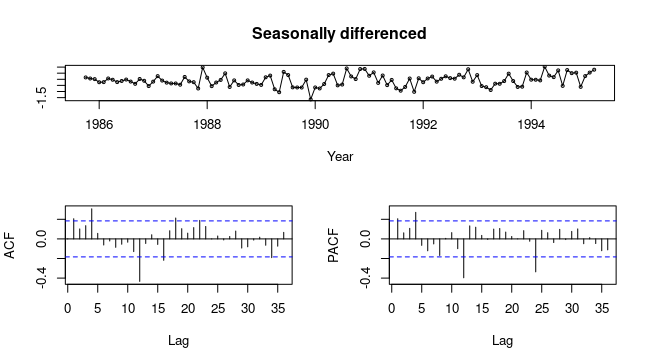
\includegraphics[scale=0.45]{fig1/data_sd1.png}
\caption{Time Domain: One step seasonal differencing}
\label{fig1:seasonal}
\end{center}
\end{figure}



\subsection{Exponential Smoothing Models}
In this part, we used both Holt-Winter and Automatic Exponential Smoothing models to fit the time series, we performed both verification and validation on the models. The best model is used to compare with the best ARIMA model and we selected the better one to forecast.

\subsubsection{Holt-Winter's Exponential Smoothing}
There are three types of exponential smoothing models in general and they are applied to different occasions. The simple exponential smoothing is used for time series without trend and seasonality, Holts' exponential smoothing model is used for time series with trend and Holt-Winter's exponential smoothing is used for time series with both trend and seasonality.  Since we found that there were seasonality within the time series and possible trend within it, we would choose to use Holt-Winter's exponential smoothing. 
\begin{table}[H]
\caption{Table: Holt-Winter's Model Parameters}
\label{table:HW}
\centering
\begin{tabular}{|c|c|c|c|c|}
\hline
a & b & s1 & s2 & s3 \\ 
1229.9643432    & 13.9814393     & 0.9426255     & 1.3041867     & 1.6756330     \\ \hline
s4 & s5 & s6 & s7 & s8 \\ 
1.5390151   & 1.3767354    &  1.0922448    &  1.0534098    &  0.7964503    \\ \hline
s9 & s10 & s11 & s12 & ~ \\  
 0.6024360     & 0.4964780   &    0.5579722    &  0.8657817   & ~ \\
\hline
\end{tabular}
\end{table}
As concluded above, the seasonal pattern was 'multiplicative', so we used Holt-Winter's exponential smoothing with 'multiplicative' mode of seasonality, and we obtained results as shown in figure \ref{fig1:HW_model}. The level, trend and seasonal parameters are shown in table \ref{table:HW}.




And the smoothing parameters are: $\alpha=0.006805899$, $\beta=1$, and $\gamma = 0.1324159$. 
% The whole fitted model is described as:
% $$\hat{x}_{t-1}^{TS}(1) = (\hat{L}_{t-1}+\hat{T}_{t-1})\cdot \hat{I}_{t-12}$$
% $$\hat{L}_{t} =0.0068(\hat{x}_{t}^{TS}/\hat{I}_{t-12})+0.9932(\hat{L}_{t-1}+\hat{T}_{t-1})$$
% $$\hat{T}_{t} =\hat{L}_{t}-\hat{L}_{t-1}$$
% $$\hat{I}_{t} = 0.1324(\hat{x}_{t}^{TS}-\hat{L}_{t})+0.8676\hat{I}_{t-12}$$
As we can see that alpha is close to zero, which means that the level update depends on much more on the past instead of recent, so the level line is smooth.  But beta=1 means that the trend update depends just on its last value, so the trend line is not smooth but it vibrates, $\gamma=0.1324159$ shows that seasonal update depends on both past and recent seasonal levels, but it depends on more on the past. 

\begin{figure}[H]
\begin{center}
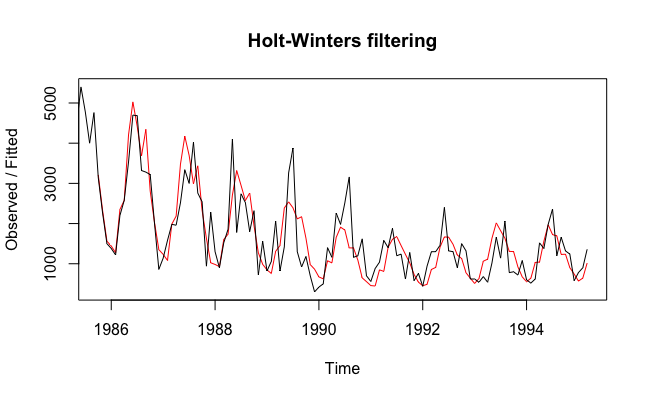
\includegraphics[scale=0.25]{fig1/data_hw_plot.png}
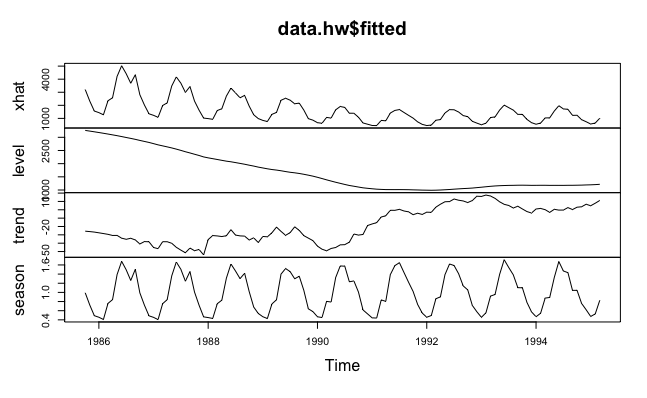
\includegraphics[scale=0.24]{fig1/data_hw_fitted.png}
\caption{Time Domain: Holt-Winter's multiplicative model}
\label{fig1:HW_model}
\end{center}
\end{figure}



To evaluate the model we obtained using Holt-Winters exponential smoothing method, we first performed verification of the model and then the validation of the model. 
To verify the model, we looked at the in-sample accuracy and the in-sample forecast errors. The in-sample accuracy is shown in table \ref{table:accuracy}, note that RMSE=552.40.
The in-sample forecast errors is shown in figure \ref{fig1:HW_forecast}.

\begin{figure}[H]
\begin{center}
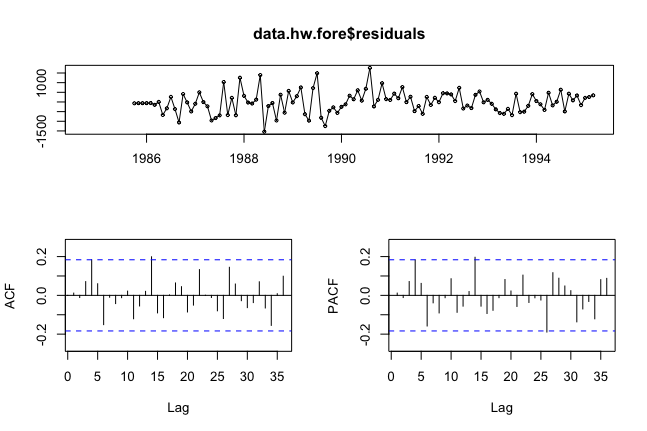
\includegraphics[scale=0.35]{fig1/HW_forecast_tsdisplay.png}
\caption{Holt-Winter's In-sample Forecast Residuals}
\label{fig1:HW_forecast}
\end{center}
\end{figure}

The ACF and PACF plots both showed that there were still some patterns within the residuals, it was not a white noise.  To see if those autocorrelations are significant or not, we performed Box-Ljung test, and from the ACF plot, there is a spike at lag=4, so we performed the test setting lag=4.


 \begin{table}[H]
 \caption{In-Sample Accuracy: Holt-Winter's}
 \label{table:accuracy}
\centering
 \begin{tabular}{|p{0.75cm}|p{0.75cm}|p{0.75cm}|p{0.75cm}|p{0.75cm}|p{0.75cm}|p{1.2cm}|}
 \hline
 ME     &  RMSE      &  MAE      &   MPE    &   MAPE   &      ACF1  & Theil's U  \\ \hline
 -6.455  & 552.40  & 419.11  & -8.015  & 31.05 & 0.0116  & 0.8196         \\
 \hline
 \end{tabular}
 \end{table}
 
 
\begin{table}[H]
\caption{Box-Ljung test}
\label{table:box_test}
\centering
\begin{tabular}{|c|}
\hline
Box-Ljung test  \\ \hline
data:  data.hw.fore\$residuals  \\  \hline
X-squared = 4.6836, df = 4, p-value = 0.3213  \\
\hline
\end{tabular}
\end{table}
The test results suggest not reject null hypothesis, meaning that the autocorrelation is not significant.  
Then we performed normality test of the residuals. The Shapiro-Wilk normality test suggested that not reject normality. So the residuals could be considered as white noise.

\begin{figure}[H]
\begin{center}
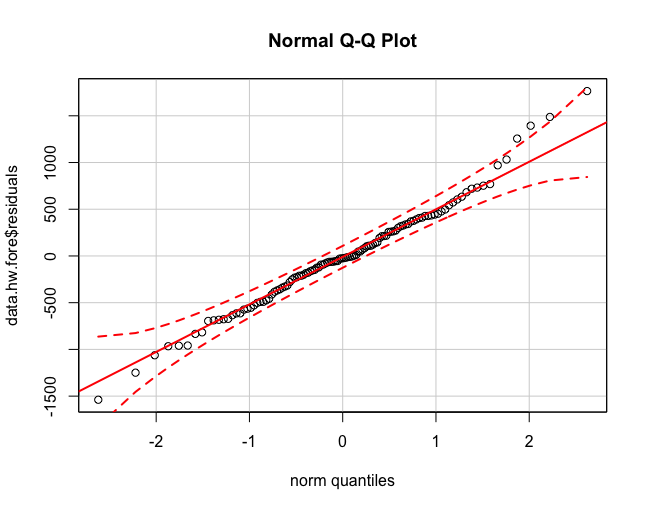
\includegraphics[scale=0.25]{fig1/qqplot.png}
\caption{Shapiro-Wilk Normality Test for Holt-Winter's Forecast Residuals}
\label{fig1:qqplot}
\end{center}
\end{figure}

\begin{table}[H]
\centering
\begin{tabular}{|c|}
\hline
Shapiro-Wilk normality test  \\  \hline
data:  data.hw.fore\$residuals  \\  \hline
W = 0.98584, p-value = 0.2759  \\
\hline
\end{tabular}
\end{table}
To validate the model, we use the last two years (19\%) data, we fit the model using data from March 1993 to March 1995. 
For the Holt-Winter's exponential smoothing model, the \textbf{RMSE} is 641.1747.

\begin{figure}[H]
\begin{center}
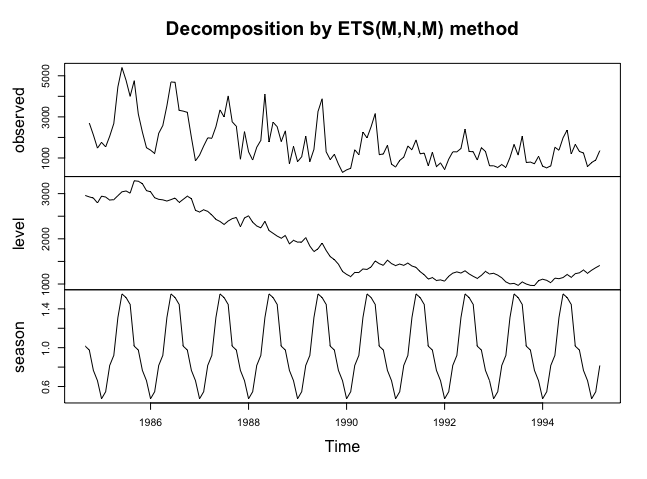
\includegraphics[scale=0.3]{fig1/ets_plot.png}
\caption{ETS Decomposition}
\label{fig1:ets_plot}
\end{center}
\end{figure}

\subsubsection{Automatic Exponential Smoothing}
As another part of exponential smoothing method, we also applied automatic exponential smoothing model to compare with the Holt-Winter's model we obtained in previous part.


\begin{figure}[H]
\begin{center}
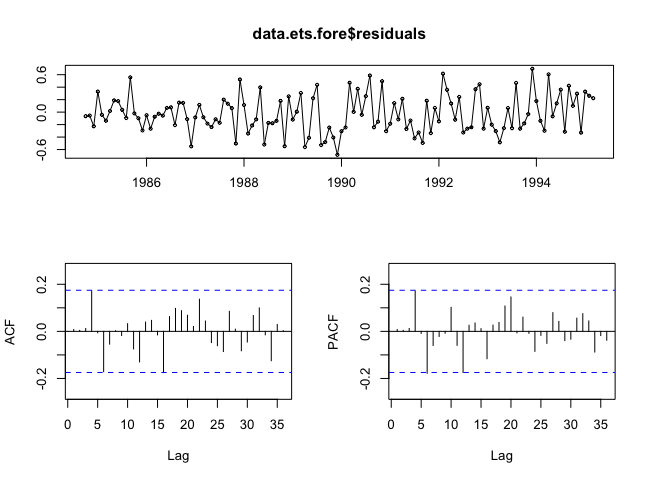
\includegraphics[scale=0.3]{fig1/est_diagnostics.png}
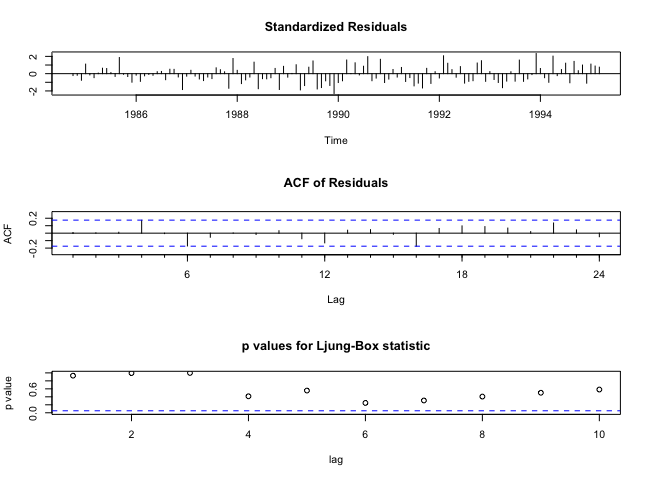
\includegraphics[scale=0.3]{fig1/ets_tsdiag.png}
\caption{ETS Model Residuals and Box-Ljung test}
\label{fig1:ets_diagnostics}
\end{center}
\end{figure}

The ETS suggests a model of ETS(M,N,M), which is multiplicative error, no trend and multiplicative seasonal pattern, and the seasonality is 12. The estimated parameters are:
$\alpha=0.1633,\gamma=1e-04$.For the initial states are:
$l=2959.0364$
$l=1.0155, , 1.4449, 1.5166, 1.5531, 1.3099, 0.9209,
           0.8169, \\0.5462, 0.4739, 0.66, 0.7661, 0.9761$,
$\sigma=0.2986$



We also performed verification for the ETS model.

 From the ACF plot we did not see any significant autocorrelations. And the Ljung-Box test statistics also showed that all autocorrelations were not significant.  The normality test for the residuals also suggests not reject null hypothesis, so the residuals could be considered as white noise.
 \begin{table}[H]
 \centering
\begin{tabular}{|c|}
\hline
Box-Ljung test  \\ \hline
data:  data.ets.fore\$residuals \\  \hline
 X-squared = 3.9444, df = 4, p-value = 0.4136  \\
\hline
\end{tabular}
\end{table}
\begin{table}[H]
\centering
\begin{tabular}{|c|}
\hline
Shapiro-Wilk normality test   \\ \hline
data:  data.ets.fore\$residuals  \\  \hline
W = 0.98269, p-value = 0.1078  \\
\hline
\end{tabular}
\end{table}
 \begin{table}[H]
 \caption{In-Sample Accuracy:ETS}
 \label{table:ets_in_accuracy}
\centering
 \begin{tabular}{|p{0.75cm}|p{0.75cm}|p{0.75cm}|p{0.75cm}|p{0.75cm}|p{0.75cm}|p{1.2cm}|}
 \hline
 ME     &  RMSE      &  MAE      &   MPE    &   MAPE   &      ACF1  & Theil's U  \\ \hline
 -67.92  & 536.14  & 417.80  & -14.42  & 30.634 & 0.6881  & -0.0232         \\
 \hline
 \end{tabular}
 \end{table}
 As shown in table \ref{table:ets_in_accuracy}, the in-sample accuracy shows the ETS model has RMSE of 536.14, which is better than the in-sample accuracy for Holt-Winter's model.
To validate the ETS model, we also used the last two years' data. The \textbf{RMSE} for the ETS model is 368.6765.

\subsubsection{Forecast}
Through verification and validation of the two exponential models, we find that ETS model performed better based on both in in-sample accuracy RMSE and validation RMSE. so we used the ETS model to forecast the future, the grey region in figure \ref{fig1:ets_forecast} is the confidence interval, the blue line is the forecast levels, the level still keeps the seasonal pattern as it goes up first and then goes down within each year, and the confidence interval reaches the biggest at peak, the exact forecast values can be found in appendix (see figure \ref{fig1:forecast_ets}). 
The exact formula for the final model is as follow, the forecast values are generated according to these formulas.
$$y_{t}=l_{t-1}s_{t-12}(1+\epsilon_{t})$$
$$l_{t}=l_{t-1}(1+0.1633\epsilon_{t})$$
$$s_{t}=s_{t-12}(1+0.0001\epsilon_{t})$$
where $\epsilon_{t}$ is the white noise with standard deviation of $\sqrt[]{0.2986}=0.5464$. As we can see from the formula, the seasonal pattern does not change much, the level changes, since 0.1633 is quite small, we can see the level does not vibrate a lot.
\begin{figure}[H]
\begin{center}
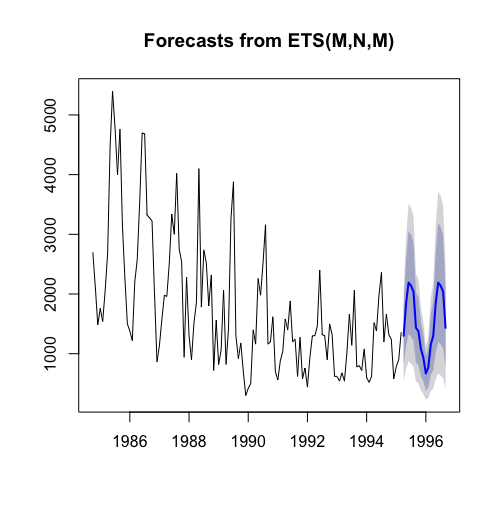
\includegraphics[scale=0.3]{fig1/ets_forecast.png}
\caption{ETS Model Forecasting}
\label{fig1:ets_forecast}
\end{center}
\end{figure}


\subsection{Box-Jenkins Model}
In this section, we used ARIMA models to fit the time series and we selected the best model according to criterion AICc. After comparing the best ARIMA model to the model we obtained in previous section, we chose the better one to forecast.
We followed the following flowchart from Hyndman's book[1] (figure \ref{fig1:flowchart}) to build a Box-Jenkins model for the time series. 

The first three steps are same as the previous section in exponential smoothing models, so we started from the fourth step. In the fourth step, we estimated the ARIMA model parameters and also came up with several candidates for it. In the plots of the seasonally differenced data, there are spikes in the PACF at lags 12 and 24, and a seasonal lag in the ACF at lag 12. This may suggest a seasonal AR(2) term. In the non-seasonal lags, there are two significant spikes in the PACF suggesting a possible AR(4) or AR(1) term. The pattern in the ACF is not indicative of any simple model. Consequently, this initial analysis suggests that a possible model for these data is an ARIMA$(4,0,0)(2,1,0)_{12}$ or ARIMA$(1,0,0)(2,1,0)_{12}$.
\begin{figure}[H]
\begin{center}
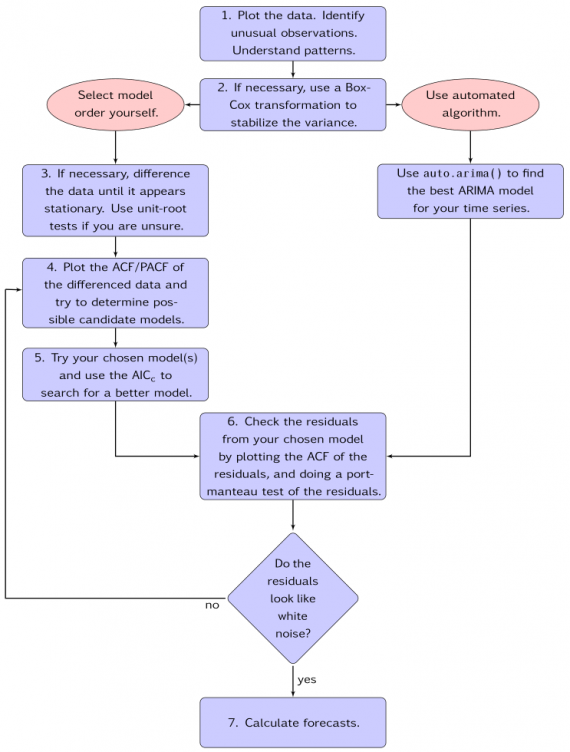
\includegraphics[scale=0.4]{fig1/flowchart.png}
\caption{Box-Jenkins Model: General process for forecasting using an ARIMA model}
\label{fig1:flowchart}
\end{center}
\end{figure}
\begin{figure}[H]
\begin{center}
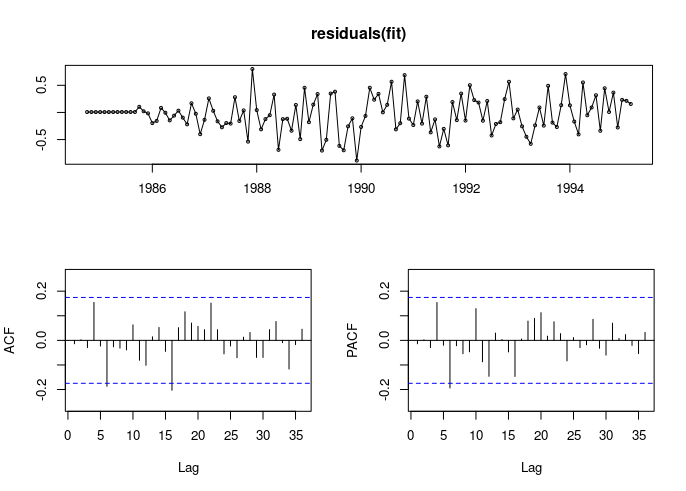
\includegraphics[scale=0.4]{fig1/bj_residuals.png}
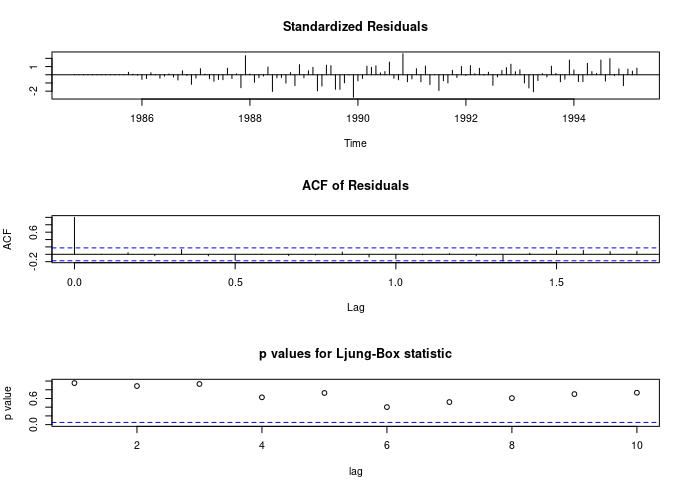
\includegraphics[scale=0.4]{fig1/test_residuals.png}
\caption{Box-Jenkins Residuals Plot}
\label{fig1:bj_residuals}
\end{center}
\end{figure}

We fitted these models along with some variations on them and computed their AICc values to verify our models which were shown in the following table \ref{table:candidate}. 


From the table \ref{table:candidate}, we selected ARIMA$(1,0,1)(2,1,0)_{12}$ which has the smallest AICc, then we look at its variants in the seasonal part, which is shown in the following table \ref{table:seasonal}.



Among all these models, the best model is ARIMA$(1,0,1)(0,1,1)_{12}$ because it has the lowest value of AICc, which is equal to 107.61. Having obtained the model, we then looked at the residuals plot, as shown in figure \ref{fig1:bj_residuals}.

\begin{table}[H]
\caption{Candidate ARIMA models and AICc}
\label{table:candidate}
\centering
\begin{tabular}{|c|c|}
\hline
Model & AICc \\ \hline
ARIMA$(4,0,0)(2,1,0)_{12}$ & 123.73  \\ 
ARIMA$(4,0,1)(2,1,0)_{12}$ &  126 \\
ARIMA$(4,0,2)(2,1,0)_{12}$ &   128.11  \\
ARIMA$(2,0,3)(2,1,0)_{12}$ & 126.76\\ 
ARIMA$(1,0,3)(2,1,0)_{12}$  & 125.07  \\ 
ARIMA$(1,0,2)(2,1,0)_{12}$ & 123.16\\ 
ARIMA$(1,0,1)(2,1,0)_{12}$ & 120.93   \\ 
ARIMA$(2,0,2)(2,1,0)_{12}$ &125.05 \\
ARIMA$(3,0,2)(2,1,0)_{12}$  & 128.16  \\ 
ARIMA$(3,0,0)(2,1,0)_{12}$ &129.03 \\
ARIMA$(2,0,0)(2,1,0)_{12}$   & 129.53  \\  
\hline
\end{tabular}
\end{table}





\begin{table}[H]
\caption{ARIMA (1,0,0) with variants in seasonal part}
\label{table:seasonal}
\centering
\begin{tabular}{|c|c|}
\hline
ARIMA Model (1,0,1) & AICc \\ \hline
ARIMA$(1,0,1)(1,1,0)_{12}$ & 134.56  \\ 
ARIMA$(1,0,1)(0,1,1)_{12}$ &  107.61  \\ 
ARIMA$(1,0,1)(1,1,2)_{12}$ & 111.81  \\ 
ARIMA$(1,0,1)(1,1,1)_{12}$ & 109.61  \\
\hline
\end{tabular}
\end{table}
As it is shown, there are significant spikes in both the ACF and PACF, but the model doesn't fail a Ljung-Box test which means the residuals are not correlated. 
There are other candidates (variants of the first estimation) which we didn't look at their AICc, so we tried running auto.arima() with differencing specified to be d=0 (trend degree of differencing) and D=1 (seasonality degree of differencing), and allowing larger models than usual. This led to an ARIMA$(1,0,1)(2,1,0)_{12}$ model (note that this model has the lowest AICc among all models with D=1 and d=0 which are invertiable too). All of its coefficients are shown in table \ref{table:autoArima}, as shown, all coefficients are significant and the obtained model did pass all the tests and residuals are like a white noise. 


\begin{table}[H]
\caption{Auto ARIMA coefficients}
\label{table:autoArima}
\centering
\begin{tabular}{|c|c|c|c|c|}
\hline
Coefficients & ar1 & ma1 & sar1 & sar2 \\ \hline
Value & 0.9636 & -0.7863 & -0.6839 & -0.3734 \\  \hline
s.e. & 0.0376 & 0.1022 & 0.0906 & 0.0869 \\
\hline
\end{tabular}
\end{table}

In addition, we tried using the automatic ARIMA algorithm. Running auto.arima() with arguments left at their default values led to an ARIMA$(0,1,5)(2,0,0)_{12}$ model. However, residuals of this model are not like white noise and its ACF and PACF have different spikes.  All in all, its AICc=135.51, which is very high compared to the previous models we studied, so we ignored this model.
\begin{figure}[H]
\begin{center}
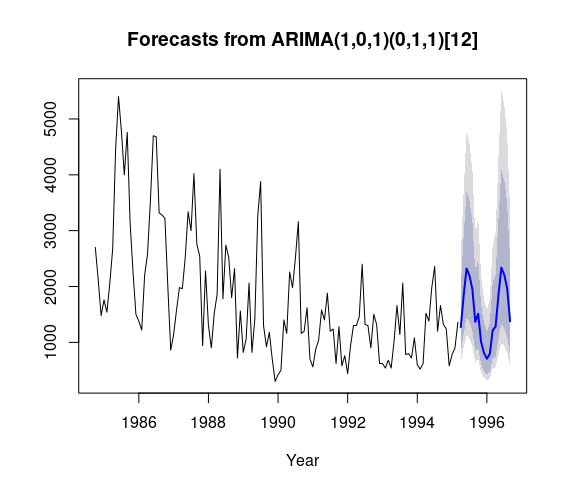
\includegraphics[scale=0.4]{fig1/forecast_BJ.png}
\caption{Box-Jenkins Forecasting}
\label{fig1:bj_forecast}
\end{center}
\end{figure}

Then we performed validation for the Box-Jenkins models, we still used the test set consisting of the last two years (19\%) of data.
Actually we performed validation for all the models listed in table \ref{table:candidate} and \ref{table:seasonal}, we found out that the \textbf{RMSE} for all models were basically the same, which means all of them are performing  the same as other candidates. Based on AICc (Verification part) and RMSE (Validation part),  ARIMA$(1,0,1)(0,1,1)_{12}$ is selected. In practice, we would normally use the best model we could find, even if it did not pass all tests.

Then we used the model ARIMA$(1,0,1)(0,1,1)_{12}$ and its coefficients (which all are significant) (Table \ref{table:ARIMA$(1,0,1)(0,1,1)_{12}$}) to forecast the next 18 months, which is shown in figure \ref{fig1:bj_forecast}. The exact forecast values can be found in appendix. (see figure \ref{fig1:forecast_box}).
The forecasted values have the seasonal pattern with a very weak increasing trend. Their prediction intervals are small at the begining, but they increase a lot at peaks, then they decreas which is obvious in both the figure \ref{fig1:bj_forecast} and in appendix (figure \ref{fig1:forecast_box}).

\begin{table}[H]
\caption{ARIMA$(1,0,1)(0,1,1)_{12}$ coefficients}
\label{table:ARIMA$(1,0,1)(0,1,1)_{12}$}
\centering
\begin{tabular}{|c|c|c|c|}
\hline
Coefficients & ar1 & ma1 & sma1 \\ \hline
Value & 0.9985 & -0.7929 & -1.0000 \\  \hline
s.e. & 0.0153 & 0.0635 & 0.1615\\
\hline
\end{tabular}
\end{table}

The specific model written in formula is as follow:
$$(1-0.9985B)(1-B^{12})x_{t}=(1-0.7929B)(1-B^{12})e_{t}$$
\begin{align*}
(1-B^{12}-0.9985B+& 0.9985B^{13})x_{t}=\\
& (1-B^{12}-0.7929B+0.7929B^{13})e_{t}
\end{align*}
\begin{align*}
x_{t}=0.9985x_{t-1}+ & x_{t-12}-0.9985x_{t-13}+ \\ & e_{t}-0.7929e_{t-1}-e_{t-12}+0.7929e_{t-13}
\end{align*}

where $\epsilon_{t}$ is the white noise with standard deviation of $\sqrt[]{0.114}=0.33763886032$.

This formula has 7 parameters and means that forecasted variable at time t depends on variable's real values and white noise at time t-1 (previous month), t-12 (previous year, the same month), and t-13 (previous year, one month before this month). 



\subsection{Comparison between Exponential Smoothing and Box-Jenkins models}
We used the two years' data (19\%) for validation for both exponential smoothing models and ARIMA models. Then we chose the same criterion to see which one performed the best.
As shown in table \ref{table:ets_arima} and figure \ref{fig1:ets_arima}, ETS model performed the best.


\begin{figure}[H]
\begin{center}
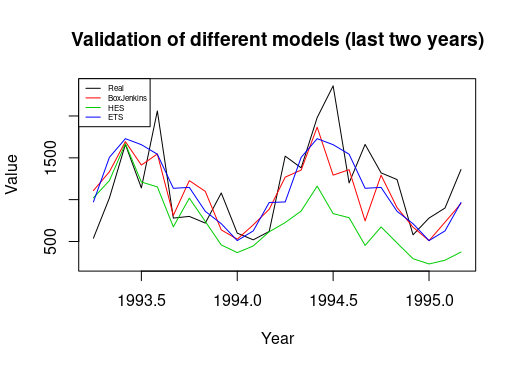
\includegraphics[scale=0.55]{fig1/ets_arima.png}
\caption{Validation Plot for Different Models}
\label{fig1:ets_arima}
\end{center}
\end{figure}


\begin{table}[H]
\caption{Validation for exponential smoothing models and ARIMA models}
\label{table:ets_arima}
\centering
\begin{tabular}{|c|c|c|c|}
\hline
metric  & Box-Jenkins  & Holt Winters& ETS\\ \hline
RMSE & 1257.881 & 641.1747  & 368.6765  \\
\hline
\end{tabular}
\end{table}



\section{Part II}

\subsection{Exploratory Data Analysis}

In this section we looked at the fingerprints of the time series. We analyzed the time series both in the time domain and the frequency domain.

\begin{figure}[H]
\begin{center}
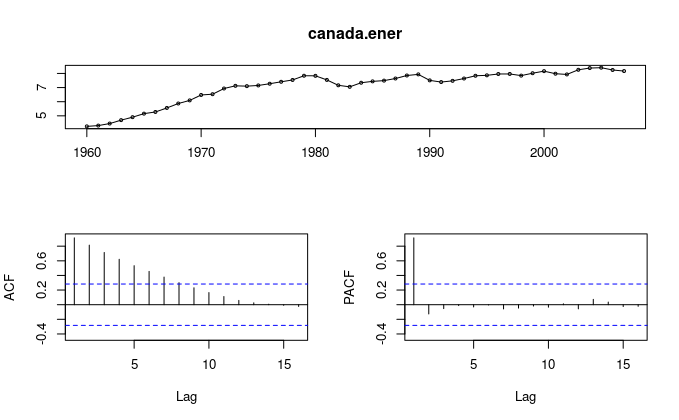
\includegraphics[scale=0.4]{fig2/tsdisplay_energy.png}
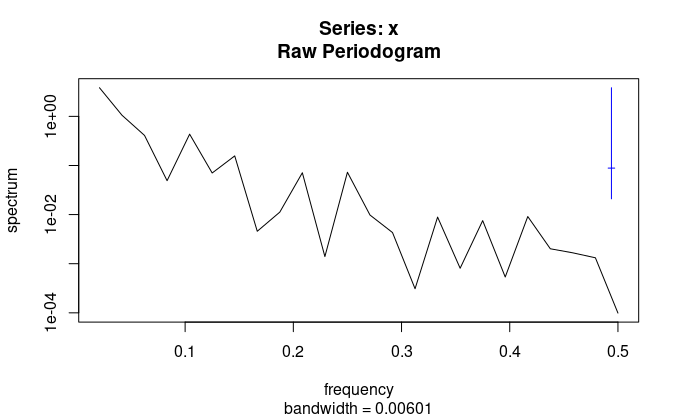
\includegraphics[scale=0.35]{fig2/period_energy.png}
\caption{Time Series Plot (energy per capita)}
\label{fig2:energy}
\end{center}
\end{figure}
Time Domain (energy per capita): The energy per capita plot shows a clearly increasing trend, but we are not sure if there is any seasonal pattern, then we looked at the tsdisplay of the capita series. The ACF plot shows a clear sign of increasing trend, but it does not suggest any seasonal pattern either.\\
Frequency domain (energy per capita): The raw periodogram shows that the dominant frequencies are in the low frequency zone, mainly smaller than 0.1, which indicates a large period. So for this time series, there is obviously a trend but there is no obvious seasonal pattern. And since there is no high frequency spikes, the time series is quite smooth.

Time domain (gdp): The gdp plot also shows an increasing trend, and it shows no obvious seasonal pattern. For the ACF and PACF plots, ACF plot has many consecutive significant correlations, which suggests the existence of an increasing trend, and it does not show any sign of a seasonal pattern.
\begin{figure}[H]
\begin{center}
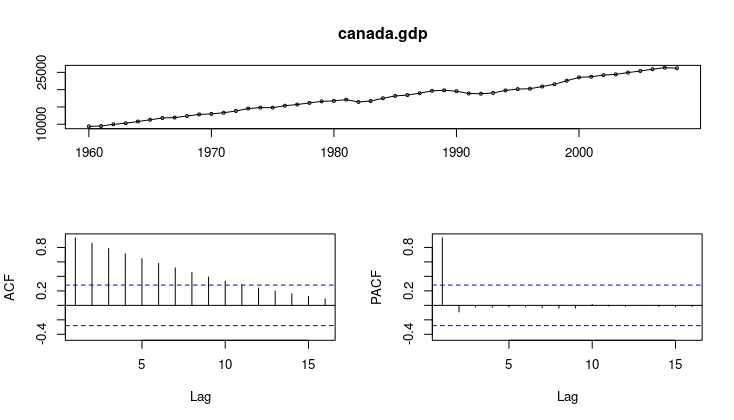
\includegraphics[scale=0.45]{fig2/tsdisplay_gdp.png}
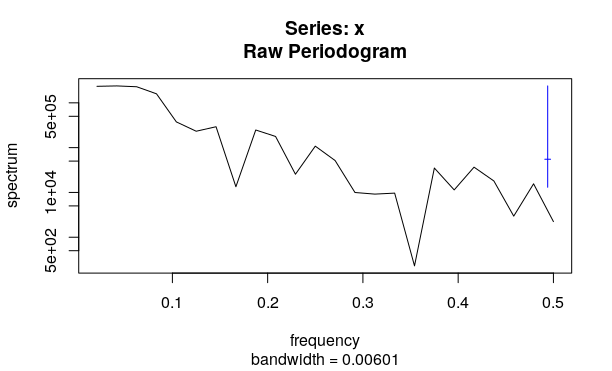
\includegraphics[scale=0.4]{fig2/periodogram_gdp.png}
\caption{Time Series Plot (gdp)}
\label{fig2:gdp}
\end{center}
\end{figure}

\begin{figure}[H]
\begin{center}
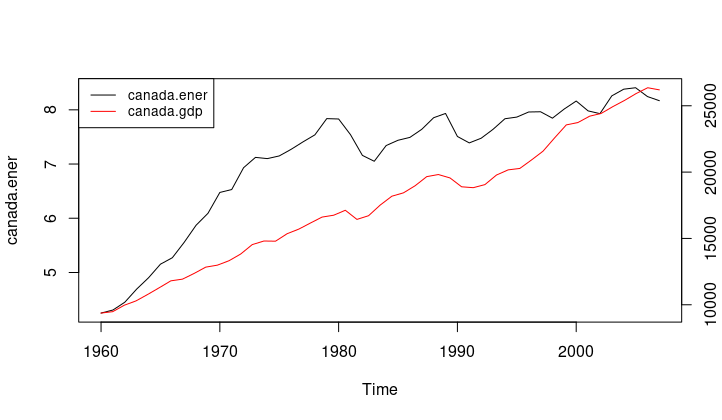
\includegraphics[scale=0.4]{fig2/both_plot.png}
\caption{Time Series Plot (energy per capita \& gdp)}
\label{fig2:both}
\end{center}
\end{figure}

Frequency domain(gdp): The raw periodogram suggests the dominant frequencies located in the low frequency zone, which indicates a very large period for the time series. So, as for the time series available, we can ignore the effect of seasonal pattern. Also because of the peaks in the low frequency zone, it shows that the time series has an increasing trend.


The time series plot for both energy per capita and gdp are shown in figure \ref{fig2:both}, it shows that both have increasing trend, this indicates a possible correlation between the two time series. 

\subsection{Univariate Box-Jenkins Model(energy per capita)}
For the Box-Jenkins model, we still followed the flowchart in figure \ref{fig1:flowchart}. The fingerprint analysis we concluded that the energy per capita time series had an increasing trend but no obvious seasonal pattern. Also since there was not much variance so we did not transform the time series. Also the time series kept increasing until 1980, after 1980, there was a slight decrease. There was no unusual changes in the time plot. (As shown in figure \ref{fig2:both})

Since the time series is not stationary, we started with one-step finite differencing.
After the one-step finite differencing,  we can see that the time series seems to be stationary. So for the ARIMA model, we choose d=1. 
Based on the ACF and PACF plots, there are spikes both at time lag 1, so we figure that the candidate for p and q should be p=1 and q=1. Since we conclude that there is no seasonal pattern, so the proposed model is ARIMA$(1,1,1)$, we also considered all other combinations of p and q and we compared all the proposed models in order to find the best one.


\begin{figure}[H]
\begin{center}
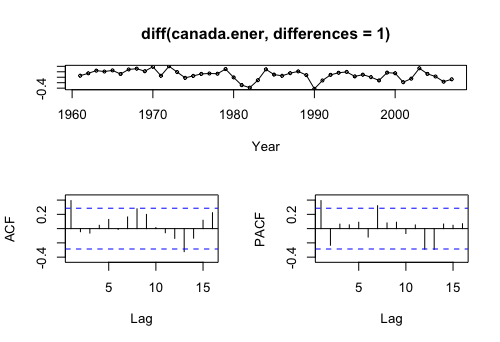
\includegraphics[scale=0.65]{fig2/diff_energy.png}
\caption{tsdisplay after one-time finite differencing( energy per capita)}
\label{fig2:finite_diff}
\end{center}
\end{figure}


\begin{table}[H]
\caption{Univariate ARIMA Models}
\label{table:univariate_arima}
\centering
\begin{tabular}{|c|c|}
\hline
Model & AICc \\ \hline
Arima(1,1,1) &  -26.45  \\ 
Arima(1,1,0) &   -27.43 \\  
Arima(1,1,2) &  -26.68  \\ 
Arima(0,1,1) &   -28.33 \\ 
Arima(0,1,0) &   -16.1 \\ 
Arima(0,1,2) &   -26.3  \\ 
Arima(2,1,0) &    -25.99 \\ 
Arima(2,1,1) &   -25.99 \\ 
Arima(2,1,2) &    -24.76\\
\hline
\end{tabular}
\end{table}



According to the AICc, ARIMA(0,1,1) gives the best model. Also by looking at the ACF and PACF plots, we could see that none of the correlations are significant. Looking at the residuals, we used qqplot as shown in figure \ref{fig2:qqplot} to check the residuals and performed Shapiro-Wilk normality test, test results suggest not reject null hypothesis, so the residuals indeed can be considered as white noise.

\begin{figure}[H]
\begin{center}
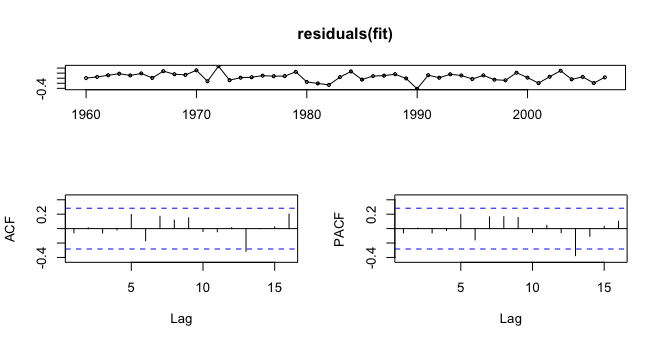
\includegraphics[scale=0.5]{fig2/univariate_residuals.png}
\caption{ARIMA: tsdisplay for the residuals (energy per capita)}
\label{fig2:residuals_univariate}
\end{center}
\end{figure}


\begin{table}[H]
\centering
\begin{tabular}{|c|}
\hline
Shapiro-Wilk normality test   \\ \hline
data:  fit.arima\$residuals \\  \hline
W = 0.98058, p-value = 0.6029  \\
\hline
\end{tabular}
\end{table}
\begin{table}[H]
\caption{ARIMA model coefficients}
\label{table:arima_coefficient}
\centering
\begin{tabular}{|c|c|c|}
\hline
Coefficients & ma1 &$\sigma^2$\\ \hline
Values & 0.5660 &0.02965\\ \hline
s.e. & 0.1357 \\
\hline
\end{tabular}
\end{table}
\begin{figure}[H]
\begin{center}
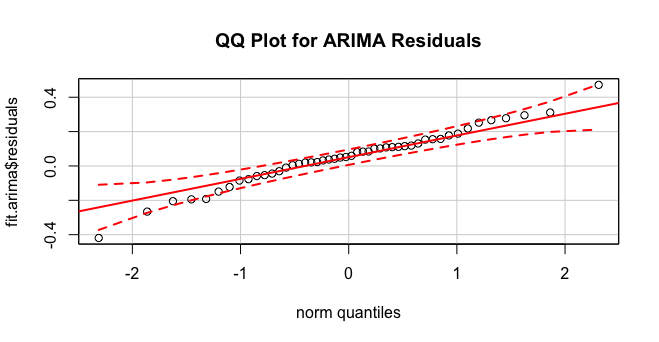
\includegraphics[scale=0.35]{fig2/can_qqplot.png}
\caption{ARIMA: QQ plot for the residuals}
\label{fig2:qqplot}
\end{center}
\end{figure}
The specific formula for the ARIMA (0,1,1) is as follow:
$$y_{t}=y_{t-1}+e_{t}+0.566e_{t-1}$$
For the non-seasonal ARIMA model,
the auto regressive part is 0 and there is a one-time finite differencing, the $e_t$ is the white noise with the standard deviation of $\sqrt[]{0.02965}=0.17219$. As we can see from the formula, the update level depends on previous value and the values of white noises at time t and time t-1 with corresponding coefficients of 1 and 0.566.

\begin{table}[H]
\caption{In-Sample Accuracy: ARIMA}
\label{table:can_arima_accuracy}
\centering
\begin{tabular}{|c|c|c|c|c|}
\hline
 ME       & RMSE       &  MAE       &  MPE      & MAPE      \\ 
0.05235639 &0.1685781& 0.1318204& 0.8583297& 1.909194   \\ \hline
MASE & ACF1 & ~ & ~ & ~ \\ 
0.7940359 &-0.05877094  & ~ & ~ & ~ \\
\hline
\end{tabular}
\end{table}

We also performed validation for the model. We found the real data for year 2008 to 2013. \cite{worldbank} And we chose the criterion \textbf{RMSE}, for the ARIMA model we obtained, the RMSE=0.3676267.

We also applied the auto.arima to select the best model automatically, and the best model suggested by auto.arima was also ARIMA(0,1,1). (See the code)




\subsection{Dynamic Regression}

We chose GDP value of Canada as the predictor variable. We took the following steps:
\begin{itemize}
\item We applied differencing until all variables (forecast and predictor) are stationary. One time differencing was enough to have stationary variables. 
\item We fitted the regression model with AR(2) errors. 
\item We calculated the errors (nt) from the fitted regression model and identified an appropriate ARMA model for them.
\item We re-fitted the entire model using the new ARMA model for the errors. 
\item  Finally, we checked that the et series looks like white noise. 
\end{itemize}


Possible candidate ARIMA models include an MA(5) and AR(1). However, further exploration reveals that an ARIMA(1,1,0) has the lowest AICc value among possible candidates. We refit the model with ARIMA(1,1,0) errors to obtain the results in table \ref{table:arima_coeff}. 
\begin{table}[H]
\caption{ARIMA model coefficients}
\label{table:arima_coeff}
\centering
\begin{tabular}{|c|c|c|}
\hline
Coefficients & ar1 & canada.gdp \\ \hline
Values & 0.3108 & 2e-04 \\ \hline
s.e. & 0.1485 & 2e-04 \\
\hline
\end{tabular}
\end{table}

The exact mathematical formula is:
$$y_{t^{'}}=0.0002x_{t}^{'}+n_{t}^{'}$$
$$n_{t}^{'}=0.3108n_{t-1}^{'}+e_{t}$$
we know that $y_{t^{'}}=y_{t}-y_{t-1}$, $x_{t^{'}}=x_{t}-x_{t-1}$, and $n_{t^{'}}=n_{t}-n_{t-1}$. We just replace them in the formula and we will have:\\
$$y_{t}-y_{t-1}=0.0002(x_{t}-x_{t-1})+0.3108(n_{t}-n_{t-1})+e_{t}$$
The final expanded formula will be:\\
$$y_{t}=y_{t-1}+0.0002x_{t}-0.0002x_{t-1}+0.3108n_{t}-0.3108n_{t-1}+e_{t}$$
and
$$n_{t}-n_{t-1}=0.3108(n_{t-1}-n_{t-2})+e_{t}$$
which is equal to:
$$n_{t}=1.3108n_{t-1}-0.3108n_{t-2}+e_{t}$$

where $\epsilon_{t}$ is the white noise with standard deviation of $\sqrt[]{0.02464}=0.15697133496$.


This formula has 6 parameters, this means that forecasted variable at time t depends on real value of forcast variable at time t-1 and value of predictor variables at time t and t-1 and white noise at time t and t-1. 

Using this model to forecast, the results is shown in figure \ref{fig2:arima_forecast}.


\begin{figure}[H]
\begin{center}
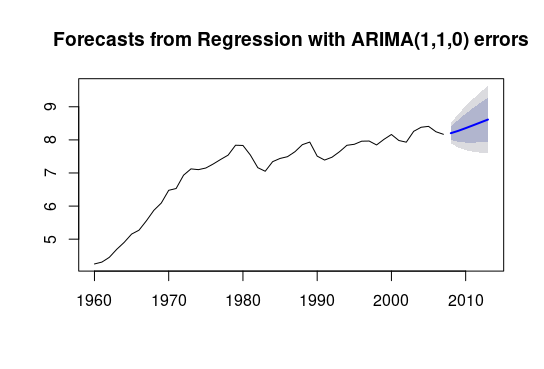
\includegraphics[scale=0.4]{fig2/arima_forecast.png}
\caption{Forecasts from Regression with ARIMA(1,1,0)}
\label{fig2:arima_forecast}
\end{center}
\end{figure}


Then we looked at the lagged version and followed the steps mentioned at section 9.1 in Hyndman's book  \cite{fpp}. We got the results shown in table \ref{table:arima_lag}.
\begin{table}[H]
\caption{Lagged Version ARIMA}
\label{table:arima_lag}
\centering
\begin{tabular}{|c|c|c|c|c|}
\hline
Coefficients & ar1 & Adlag0 & Adlag1 & Adlag2 \\ \hline
Values & 0.3592 & 2e-04 & 1e-04 & -1e-04 \\ \hline
s.e. & 0.1786 & 2e-04 & 2e-04 & 2e-04 \\
\hline
\end{tabular}
\end{table}
The chosen model includes GDP only the last three months and has AR(1) errors. The model can be written as:
$$y_{t}^{'}=0.0002x_{t}^{'}+0.0001x_{t-1}^{'}-0.0001x_{t-2}^{'}+n_{t}^{'}$$
$$n_{t}^{'}=0.3592n_{t-1}^{'}+e_{t}$$
Notice that $y_{t}^{'}=y_{t}-y_{t-1}$ and so on.
So the expanded version of the formula is as following:
\begin{align*}
y_{t}-y_{t-1}&=0.0002(x_{t}-x_{t-1})+ 0.0001(x_{t-1}-x_{t-2})- \\ & 0.0001(x_{t-2}-x_{t-3})+(n_{t}-n_{t-1})
\end{align*}
which is equal to:
\begin{align*}
y_{t}=y_{t-1}&+0.0002x_{t}-0.0001x_{t-1}-\\ & 0.0002x_{t-2}-0.0001x_{t-3}+n_{t}-n_{t-1}
\end{align*}
and 
$$n_{t}-n_{t-1}=0.3592(n_{t-1}-n_{t-2})+e_{t}$$
which is equal to:
$$n_{t}=1.3592n_{t-1}-0.3592n_{t-2}+e_{t}$$

where $\epsilon_{t}$ is the white noise with standard deviation of $\sqrt[]{0.02318}=0.15224979474$.


This formula means that forecasted variable at time t depends on real value of forcast variable at time t-1 and value of predictor variables at time t, t-1, t-2, and t-3. In addition, it depends on white noise at time t and t-1.

Using this model to forecast, the results is shown in figure \ref{fig2:arima_forecast_gdp}.



For the forecasting part, first we forecasted the next 8 years of the predictor variable using ets command in R, then we used the result to forecast the forecast variable using dynamic regression. 

Validation and verification of these two models are shown in table \ref{table:DR_verification_validation}




\begin{figure}[H]
\begin{center}
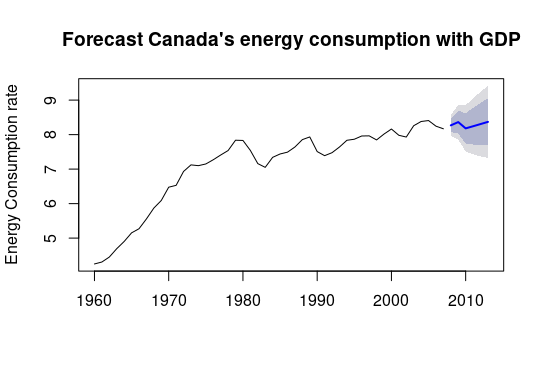
\includegraphics[scale=0.4]{fig2/arima_forecast_gdp.png}
\caption{Forecasts Canada's Energy with GDP}
\label{fig2:arima_forecast_gdp}
\end{center}
\end{figure}



\begin{table}[H]
\caption{Verification and Validation of Dynamic Regression models}
\label{table:DR_verification_validation}
\centering
\begin{tabular}{|c|c|c|}
\hline
Models & Dynamic Regression (Simple) & Dynamic Regression (Lagged) \\ \hline
Verification & -36.06 (AICc) & -32.14 (AICc) \\ \hline
Validation & 0.613 (RMSE) & 0.472 (RMSE) \\
\hline
\end{tabular}
\end{table}
Based on the outputs, there is no single model which outperforms in both verification and validation parts, but we choose the lagged version as our final model here because it perfroms better in the validation part.

\subsection{Exponential Smoothing models}
We used non-seasonal exponential smoothing model for energy indicator of Canada. 
There are two ways to do this in R, we could choose either HoltWinters command or ets one. We did both and chose the best one. 
First, we ran with HoltWinters with gamma=FALSE because the time series doesn't contain seasonality.  Other parameters are obtained using optimizing automatically.  We obtained $\alpha=1, \beta=0, \gamma=FALSE$

For level, it only takes the recent value. For trend, it only takes the difference of levels into account.
 \begin{table}[H]
 \caption{In-Sample Accuracy: Holt-Winter's ES}
 \label{table:accuracy_in}
\centering
 \begin{tabular}{|p{0.75cm}|p{0.75cm}|p{0.75cm}|p{0.75cm}|p{0.75cm}|p{0.75cm}|p{1.2cm}|}
 \hline
 ME     &  RMSE      &  MAE      &   MPE    &   MAPE   &      ACF1  & Theil's U  \\ \hline
 0.02761  & 0.1851  & 0.1467  & 0.5440  & 2.113 & 0.3937  & 0.8849       \\
 \hline
 \end{tabular}
 \end{table}
Next we fit the time series with ETS model. We obtained $\alpha=0.9999, \beta=0.1217$.
 ETS gave us a non-seasonal model with additive trend and multiplicative error. Its alpha is close to 1 which means the last level and last trend have more weights when it wants to predict next level and trend. 
  \begin{table}[H]
 \caption{In-Sample Accuracy: ETS}
 \label{table:accuracy_in_ets}
\centering
 \begin{tabular}{|p{0.75cm}|p{0.75cm}|p{0.75cm}|p{0.75cm}|p{0.75cm}|p{0.75cm}|p{1.2cm}|}
 \hline
 ME     &  RMSE      &  MAE      &   MPE    &   MAPE   &      ACF1  & Theil's U  \\ \hline
 -0.027  & 0.1761  & 0.1327  & -0.359  & 1.8535 & 0.7993  & 0.2757      \\
 \hline
 \end{tabular}
 \end{table}
 \textbf{Based on RMSE metrics, ETS performs better, so we choose ETS one and forecast next 6 years}, as shown in figure \ref{fig2:can_ets_forecast}.
 
The exact mathematical formulas for ETS model are:
 $$y_{t}=(L_{t-1}+T_{t-1})(1+\epsilon_{t})$$
$$L_{t}=(L_{t-1}+T_{t-1})(1+0.9999\epsilon_{t})$$
$$T_t=T_{t-1}+0.1217(L_{t-1}+T_{t-1})\epsilon_{t}$$
\\

 where $\epsilon_{t}$ is the white noise with standard deviation of $\sqrt[]{0.0235}=0.15329709716$.

Here, we have a Holt’s linear method or ETS(M,A,N) with multiplicative errors which means a multiplicative error, an additive trend, and no seasonality. The forecasted variable is sum of the last trend and level multiplied by $1+\epsilon_{t}$. The level depends on the previous level and trend multiplied by $1+0.9999\epsilon_{t}$. The trend depends on the previous level and trend and error value at time $t$.
 
 


 \begin{figure}[H]
\begin{center}
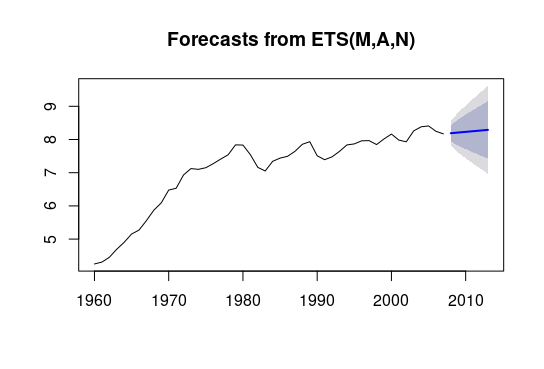
\includegraphics[scale=0.4]{fig2/can_ets_forecast.png}
\caption{Forecasts Using ETS}
\label{fig2:can_ets_forecast}
\end{center}
\end{figure} 
 
\subsection{Comparison between the models}
We used the real values from 2008 to 2013 to validate all models [2]. Based on RMSE, the Box-Jenkins model performed the best. However when we plotted the forecast by all models with the real values in the same figure (figure \ref{fig2:validation_plot}), we found out that all models did not work, all predictions are basically increasing while the real value is decreasing.

\begin{figure}[H]
\begin{center}
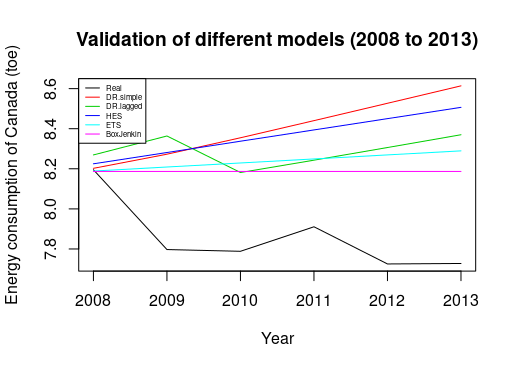
\includegraphics[scale=0.4]{fig2/validation_plot.png}
\caption{Validation plot of all models}
\label{fig2:validation_plot}
\end{center}
\end{figure}

\begin{table}[H]
\begin{tabular}{|c|c|c|c|p{0.8cm}|p{0.6cm}|}
\hline
metric & Box-Jenkins & DR(Simple) & DR(Lagged) & ES(HW) & ETS \\ \hline
RMSE & 0.367 & 0.613 & 0.472 & 0.563 & 0.426 \\
\hline
\end{tabular}
\end{table}



We tried to think about the reason why the forecast did not work and we thought about the global financial crisis.
Obviously, due to unusual financial crisis in 2008, energy per capita and gdp both decreased while the predictions can not capture this.  

So as we can see, even if we tried to build the best model possible, still there are some incidents that may affect the real time series data, and we can not build perfect model using different time series models.

\section{Discussion}
Time series analysis is technically flexible in the sense that there are several methods to build a model for a time series. Among all these models, we do follow some 'principles', for example, we always start analysis with the exploratory data analysis of the time series, choosing the appropriate parameters according to ACF and PACF, verification and validation are both necessary when building the models.

After writing this report, we found out that there was no golden hammer for all datasets. In addition, the tools available sometimes do not work as the way we thought they would be. For example, in the energy consumption part, we tried different models but the error was not acceptable and always very big. We also found out that even if we found the best model possible, sometimes it was still very difficult for the predictions to comply with the real data, simply because there are some patterns or incidents which the models can not capture.


\begin{thebibliography}{5}
\bibitem{time_series}
\url{https://en.wikipedia.org/wiki/Time_series}
	\bibitem{fpp} 
	Hyndman, Rob J., and George Athanasopoulos. Forecasting: principles and practice. OTexts, 2014.
    	\bibitem{worldbank} 
\url{http://data.worldbank.org/indicator/EG.USE.PCAP.KG.OE?locations=CA, accessed July 26, 2017.}
\end{thebibliography}


\newpage

\begin{appendix}


\begin{figure}[H]
\begin{center}
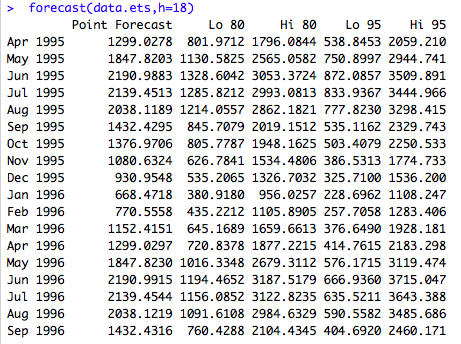
\includegraphics[scale=0.55]{fig1/forecast.png}
\caption{Forecast Using ETS model}
\label{fig1:forecast_ets}
\end{center}
\end{figure}


\begin{figure}[H]
\begin{center}
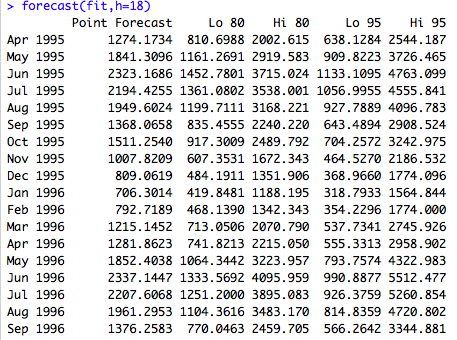
\includegraphics[scale=0.55]{fig1/forecast_box.png}
\caption{Forecast Using Box-Jenkins model}
\label{fig1:forecast_box}
\end{center}
\end{figure}
\newpage
\begin{lstlisting}[language=R,basicstyle=\tiny]
PART I
########################
library('fpp')
library('ggplot2')
library('forecast')
library(car)

##### importing and transforming the dataset
data.ts <- ts(group04_data_1$month04, start=c(1984,10),
end = c(1995,3),frequency=12)

######## exploratory data analysis part
###time domain
plot(data.ts)

tsdisplay(data.ts)

seasonplot(data.ts, season.labels = TRUE, year.labels = TRUE, col=rainbow(12))

monthplot(data.ts)

data.log <- log(data.ts)
plot(data.log)

######### seasonal decomposition
data.sd1 <- diff(data.ts, lag=12, differences = 1)
plot(data.sd1)

data.sd2 <- diff(data.ts, lag=12, differences = 2)
tsdisplay(data.sd2)
plot(data.sd2)

data.deco <- decompose(data.ts,type = 'additive')
plot(data.deco)

data.deco.mul <- decompose(data.ts,type = 'multiplicative')
plot(data.deco.mul)


###frequency domain
spectrum(data.ts)
spectrum(data.ts, span=5)
#spectrum(data.sd1)
#spectrum(data.sd2)


######### exponential smoothing model
#Holt-Winter's exponential smoothing
data.hw <- HoltWinters(data.ts,seasonal = 'multiplicative')
plot(data.hw)

#model parameter
data.hw$alpha
data.hw$beta
data.hw$gamma
data.hw$coefficients

data.hw$fitted
plot(data.hw$fitted)
data.hw$SSE
with(data.hw,accuracy(fitted,x))



#diagnostics
data.hw.fore <- forecast(data.hw)
tsdisplay(data.hw.fore$residuals)
#from the ACF plot, it looks like the lag is 4.
Box.test(data.hw.fore$residuals,lag = 4, type = 'Ljung-Box')
qqPlot(data.hw.fore$residuals, main = 'Normal Q-Q Plot')
shapiro.test(data.hw.fore$residuals)


#validation
exvalidate <- function(x, h,...)
{
  train.end <- time(x)[length(x)-h]
  test.start <- time(x)[length(x)-h+1]
  train <- window(x,end=train.end)
  test <- window(x,start=test.start)
  fit <- HoltWinters(train,...)
  fc <- forecast.HoltWinters(fit,h)
  return(accuracy(fc,test)[2,"RMSE"])
  #return(fc)
}
exvalidate(data.ts, h=24, alpha=0.08586768,beta=0,gamma=0.4719598,
seasonal='multiplicative')

#HES_plot <- exvalidate(data.ts, h=24, alpha=0.08586768,beta=0,
gamma=0.4719598, seasonal='multiplicative')$mean


#automatic exponential smoothing
data.ets <- ets(data.ts)
summary(data.ets)
plot(data.ets)
accuracy(data.ets)
tsdiag(data.ets)
data.ets$aicc
data.ets.fore <- forecast.ets(data.ets,h=18)
#data.ets.fore
#plot(data.ets.fore)
#normality test
tsdisplay(data.ets.fore$residuals)
Box.test(data.ets.fore$residuals, lag = 4, type='Ljung-Box')
qqPlot(data.ets.fore$residuals)
shapiro.test(data.ets.fore$residuals)

with(data.ets,accuracy(fitted,x))
#validation
etsvalidate <- function(x,h)
{
  train.end <- time(x)[length(x)-h]
  test.start <- time(x)[length(x)-h+1]
  train <- window(x,end=train.end)
  test <- window(x,start=test.start)
  fit <- ets(train)
  fc <- forecast.ets(fit,h)
  return(accuracy(fc,test)[2,"RMSE"])
  #return(fc)
}
etsvalidate(data.ts,h=24)

#ets_plot <- etsvalidate(data.ts,h=24)$mean

#forecast
data.ets.fore <- forecast(data.ets,h=18)
plot(data.ets.fore)

#log transform
data.log <- log(data.ts)
plot(data.log)
data.log.hw <- HoltWinters(data.log,seasonal = 'additive')
plot(data.log.hw)
data.hw <- HoltWinters(data.ts,seasonal = 'additive')



######### Box-Jenkins model

plot(data.ts)

tsdisplay(data.ts)

data.log <- log(data.ts)

plot(data.log)

tsdisplay(data.log)

tsdisplay(diff(data.log,12), main="Seasonally differenced", xlab="Year")

### choosing the best model AICc
fit <- Arima(data.ts, order=c(1,0,1), seasonal=c(0,1,1),lambda = 0)
qqPlot(fit$residuals)
accuracy(fit)
tsdiag(fit)

tsdisplay(residuals(fit))
Box.test(residuals(fit),lag=36, fitdf = 4,type="Ljung-Box")

#data.d1 <- diff(data.ts, differences = 1)

#data.d1.sd2 <- diff(data.d1, lag=12, differences = 2)


#tsdisplay(data.d1)

#data.d2 <- diff(data.ts, differences = 2)

#data.d2.sd1 <- diff(data.d2, lag=12, differences = 1)

#tsdisplay(data.d2.sd1)

auto.arima(data.ts)

fit <- auto.arima(data.ts, lambda=0, d=0, D=1,ic="aicc" ,
max.order=10, stepwise=FALSE, approximation=FALSE)
tsdisplay(residuals(fit))
Box.test(residuals(fit), lag=36, fitdf=8, type="Ljung")


#####################
getrmse <- function(x,h,...)
{
  train.end <- time(x)[length(x)-h]
  test.start <- time(x)[length(x)-h+1]
  train <- window(x,end=train.end)
  test <- window(x,start=test.start)
  fit <- Arima(train,...)
  fc <- forecast(fit,h=h)
  return(accuracy(fc,test)[2,"RMSE"])
  #return(fc)
}

getrmse(data.ts,h=24,order=c(3,0,0),seasonal=c(2,1,0),lambda=0)

#BoxJenkins_plot <- getrmse(data.ts,h=24,order=c(3,0,0),
seasonal=c(2,1,0),lambda=0)$mean

### null-hypothesis = stationary time series
kpss.test(data.ts)

### ndiffs
ns <- nsdiffs(data.ts)
if(ns > 0) {
  xstar <- diff(data.ts,lag=frequency(data.ts),differences=ns)
} else {
  xstar <- data.ts
}
nd <- ndiffs(xstar)
if(nd > 0) {
  xstar <- diff(xstar,differences=nd)
}

plot(xstar)

x<-data.ts
h=24
test.start <- time(x)[length(x)-h+1]
real <- window(x,start=test.start)

#Plot (validation of different models)
ts.plot(real,BoxJenkins_plot,HES_plot,ets_plot,col=1:4,
gpars = list(ylab="Value",xlab="Year"))
#col=c("black","red","green","blue","pink"))
title(main = "Validation of different models (last two years)")

legend("topleft",           
       legend=c("Real","BoxJenkins","HES","ETS"), 
       col=1:4,
       lty=1,              
       cex=0.5)



PART II
#########################
library(fpp)
library(ggplot2)
library(forecast)
library(reshape)
library(car)
##Exploratory Analysis

canada.ener <- ts(group04_data_2$ener_canada, start=1960,end=2007)

plot(canada.ener, main='Energy per Capita Plot')

tsdisplay(canada.ener)

spectrum(canada.ener)
spectrum(canada.ener, span=5)
canada.ener.d1 <- diff(canada.ener, differences = 1)
tsdisplay(canada.ener.d1)
plot(canada.ener.d1,main='Finite Differencing Energy per Capita')

#canada.ener.d2 <- diff(canada.ener, differences = 2)
#tsdisplay(canada.ener.d2)
#plot(canada.ener.d2,main='Two Steps Finite Differencing Energy per Capita')

plot(cbind(canada.ener,canada.gdp), main='')
########

canada.gdp <- ts(group04_data_2$gdp_canada, start=1960,end=2007)

plot(canada.gdp)

tsdisplay(canada.gdp)

spectrum(canada.gdp)

canada.gdp.d1 <- diff(canada.gdp, differences = 1)
tsdisplay(canada.gdp.d1)
plot(canada.gdp.d1)

#canada.gdp.d2 <- diff(canada.gdp, differences = 2)
#tsdisplay(canada.gdp.d2)
#plot(canada.gdp.d2)

### Plot together
plot(canada.ener, las=0)
par(new=TRUE)               
plot(canada.gdp,
     col=2,
     bty='n',               
     xaxt="n",               
     yaxt="n",              
     xlab="", ylab="")

axis(4, las=0)

legend("topleft",           
       legend=c("canada.ener","canada.gdp"), 
       col=1:2,
       lty=1,              
       cex=0.85)
############## Box-Jekins ARIMA model
plot(canada.ener) #variance not much, do not need to transform
tsdisplay(canada.ener)
tsdisplay(diff(canada.ener,differences = 1), xlab="Year")

# choose the best model according to AICc, other models are omitted, 
# see the results table in the report
fit.arima <- Arima(canada.ener, order=c(0,1,1), method = 'ML')
summary(fit.arima)

qqPlot(fit.arima$residuals)
shapiro.test(fit.arima$residuals)
accuracy(fit.arima)
tsdisplay(residuals(fit.arima))

fit <- auto.arima(canada.ener,d=1,D=0,ic='aicc')
summary(fit)
tsdisplay(residuals(fit))

canada.ener.boxjenkin.fore <- forecast.Arima(fit.arima,h=6)
canada.ener.boxjenkin.fore$mean



############## Dynamic Regression 
#first, we should remove trend and seasonality? d=1

#First check
(fit <- Arima(canada.ener, xreg=canada.gdp,order=c(2,1,0)))
tsdisplay(arima.errors(fit), main="ARIMA errors")
tsdisplay(residuals(fit)) #seems like a white noise

##check candidates
(fit_simple <- Arima(canada.ener, xreg=canada.gdp,order=c(1,1,0)))
tsdisplay(residuals(fit_simple)) #seems like a white noise
Box.test(residuals(fit_simple),fitdf=1,lag=5,type="Ljung")
canada.gdp.ets <- ets(canada.gdp)
canada.gdp.ets.fore <- forecast(canada.gdp.ets, h=6)
plot.forecast(canada.gdp.ets.fore)

canada.gdp.next <- canada.gdp.ets.fore$mean

DR.simple.fore <- forecast(fit_simple,xreg=canada.gdp.next, h=6)
plot.forecast(DR.simple.fore)

# Lagged predictors. Test 0, 1, 2 or 3 lags.
Advert <- cbind(canada.gdp,
                c(NA,canada.gdp[1:47]),
                c(NA,NA,canada.gdp[1:46]),
                c(NA,NA,NA,canada.gdp[1:45]))
colnames(Advert) <- paste("AdLag",0:3,sep="")

# Choose optimal lag length for advertising based on AIC
# Restrict data so models use same fitting period
fit1 <- auto.arima(canada.ener[4:48], xreg=Advert[4:48,1], d=1)
fit2 <- auto.arima(canada.ener[4:48], xreg=Advert[4:48,1:2], d=1)
fit3 <- auto.arima(canada.ener[4:48], xreg=Advert[4:48,1:3], d=1)
fit4 <- auto.arima(canada.ener[4:48], xreg=Advert[4:48,1:4], d=1)
fit5 <- auto.arima(canada.ener[4:48], xreg=Advert[4:48,2], d=1)
fit6 <- auto.arima(canada.ener[4:48], xreg=Advert[4:48,2:3], d=1)
fit7 <- auto.arima(canada.ener[4:48], xreg=Advert[4:48,2:4], d=1)
fit8 <- auto.arima(canada.ener[4:48], xreg=Advert[4:48,3], d=1)
fit9 <- auto.arima(canada.ener[4:48], xreg=Advert[4:48,3:4], d=1)

# Best model fitted to all data (based on AICc)
# Refit using all data
(fit_lagged <- auto.arima(canada.ener, xreg=Advert[,1:3], d=1))

#forecasting
DR.lagged.fore <- forecast(fit_lagged, xreg=cbind(canada.gdp.next[1:6],
c(Advert[47,1],canada.gdp.next[2:6])
,c(Advert[46,2],Advert[47,2],canada.gdp.next[3:6])), h=6)

plot(DR.lagged.fore, main="Forecast Canada's energy consumption with GDP", 
ylab="Energy Consumption rate")

##CCF part
ccf(canada.ener,canada.gdp,na.action = na.omit)
ccf(canada.ener.d1,canada.gdp.d1,na.action = na.omit)


###################################
#Exponential Smoothing
plot(canada.ener)
canada.ener.hes <- HoltWinters(canada.ener, gamma = FALSE)

plot(canada.ener.hes$fitted)
plot(canada.ener.hes)

canada.ener.hes$SSE
with(canada.ener.hes, accuracy(fitted,x))

canada.ener.hes.fore <- forecast.HoltWinters(canada.ener.hes,h=6)
plot.forecast(canada.ener.hes.fore)

ggtsdisplay(canada.ener.hes.fore$residuals)
accuracy(canada.ener.hes.fore)

#automatic exponential smoothing
canada.ener.ets <- ets(canada.ener)
summary(canada.ener.ets)
plot(canada.ener.ets)
accuracy(canada.ener.ets)
tsdiag(canada.ener.ets)
canada.ener.ets.fore <- forecast.ets(canada.ener.ets,h=6)
canada.ener.ets.fore
plot(canada.ener.ets.fore)
#normality test
tsdisplay(canada.ener.ets.fore$residuals)
Box.test(canada.ener.ets.fore$residuals, lag = 4, type='Ljung-Box')
qqPlot(canada.ener.ets.fore$residuals)
shapiro.test(canada.ener.ets.fore$residuals)

###Validation part

RMSE = function(m, o){ #m stands for model and o stands for observation
  sqrt(mean((m-o)^2))
}

canada.ener_future<-read.csv("Dropbox/TSFproject/canada - Sheet1.csv")
canada.ener_future <- canada_Sheet1
RMSE(canada.ener.boxjenkin.fore$mean,canada.ener_future$energy)
RMSE(DR.simple.fore$mean,canada.ener_future$energy)
RMSE(DR.lagged.fore$mean,canada.ener_future$energy)
RMSE(canada.ener.hes.fore$mean,canada.ener_future$energy)
RMSE(canada.ener.ets.fore$mean,canada.ener_future$energy)

#Plot (validation of different models)
ts.plot(canada.ener_future$energy,DR.simple.fore$mean,DR.lagged.fore$mean,
canada.ener.hes.fore$mean,canada.ener.ets.fore$mean,canada.ener.boxjenkin.fore$mean,
col=1:6,gpars = list(ylab="Energy consumption of Canada (toe)",xlab="Year"))
#col=c("black","red","green","blue","pink"))
title(main = "Validation of different models (2008 to 2013)")

legend("topleft",           
       legend=c("Real","DR.simple","DR.lagged","HES","ETS","BoxJenkin"), 
       col=1:6,
       lty=1,              
       cex=0.48)

\end{lstlisting}  
\end{appendix}

\end{document}